\subsection{Apéndice A : Algoritmos}

\subsubsection{Algoritmo para eliminar Frames Intermedios} \label{eliminarframes}

\lstset{language=C++, breaklines=true, basicstyle=\footnotesize}
\begin{lstlisting}[frame=single]
void eliminarFrames (Parametros &params){

	assert(params.framesIntermedios < (params.frames -2));

	params.output << (params.frames/(params.framesIntermedios+1)) + ( (params.frames % (params.framesIntermedios+1) != 0) ? 1 : 0 ) << std::endl;
	params.output << params.height << " " << params.width << std::endl;
	params.output << params.framerate << std::endl ;

	int k = 0;
	int i, j;

	vector<vector<int> >* frame = new vector<vector<int>>(params.height, vector<int>(params.width));

	while (k < params.frames){
		if (k % (params.framesIntermedios+1) == 0 ){
			//Cargo la imagen actual
			for (i=0; i < params.height; i++){
				for (j=0; j < params.width; j++){
				params.input >> (*frame)[i][j];
				}
			}
			imprimirFrame(params.output, *frame, params.height, params.width);
		}else{
			// tiro el frame
			for (i=0; i < params.height; i++){
				//ignoro la linea
				//params.input.ignore(std::numeric_limits<std::streamsize>::max(), '\n');
				for (j=0; j < params.width; j++){
					params.input >> (*frame)[i][j];
					}
				}
			}
		k++;
	}
	delete frame;
}
\end{lstlisting}

\subsubsection{Algoritmo para calcular ECM} \label{ecmalgo}

\lstset{language=C++, breaklines=true, basicstyle=\footnotesize}
\begin{lstlisting}[frame=single]
double ecm (Parametros &params, Parametros &params2){
	assert(params.height == params2.height);
	assert(params.width == params2.width );
	int frames = (params.frames <= params2.frames) ? params.frames : params2.frames;
	double promedio = 0;
	double ecm;
	double max = 0;
	int i,j,k;
	
	vector<vector<double> >* frameA = new vector<vector<double>>(params.height, vector<double>(params.width));
	vector<vector<double> >* frameB = new vector<vector<double>>(params.height, vector<double>(params.width));

	for (k=0; k< 5; k++){
		//cargo Frame A
		for (i=0; i < params.height; i++){
			for (j=0; j < params.width; j++){
			params.input >> (*frameA)[i][j];
			}
		}
		//cargo Frame B
		for (i=0; i < params.height; i++){
			for (j=0; j < params.width; j++){
			params2.input >> (*frameB)[i][j];
			}
		}
		ecm = 0;
		for (i=0; i < params.height; i++){
			for (j=0; j < params.width; j++){
				ecm +=  pow ( abs( (*frameA)[i][j] - (*frameB)[i][j] ), 2);
			}
		}
		promedio += ecm; //sumo el ecm sin haberlo dividido por el mn , lo divido al final una vez sumados todos
		ecm = ecm / (params.width * params.height);
		//Imprimo ECM del frame k
		cout << "ECM frame " << k << ": " << ecm << std::endl ;
  		max = (ecm > max) ? ecm : max ;
		
	}
	promedio = promedio / (params.width * params.height);
	promedio = promedio / frames;
	params.output << "ECM promedio: " << promedio << std::endl;
	params.output << "Maximo error obtenido: " << max << std::endl;
	return promedio;

}
\end{lstlisting}

\newpage

\subsection{Apéndice B: Resultados cuantitativos sobre ECM y PSNR} \label{cuant}

La siguiente tabla muestra el ECM promedio obtenido con cada algoritmo para cada input, según la cantidad de frames internos (FI) eliminados: 

\bigskip
\captionof{table}{ECM: Promedios}
\begin{tabular}{| c | c | c | c | c | c | c | c |} 
\hline
\textbf{Método} & \textbf{FI} & \textbf{cupcake} & \textbf{perro} & \textbf{morocho} & \textbf{tenis} & \textbf{bebes} & \textbf{fideos} \\ 
\hline
Vecino Más Cercano & 2 & 45.0112 & 314.75 & 83.308 & 30.9356 & 120.327 & 61.5792 \\ 
\hline
Vecino Más Cercano & 4 & 75.0243 & 571.526 & 122.311 & 60.5956 & 201.26 & 116.639 \\ 
\hline
Vecino Más Cercano & 6 & 91.8027 & 762.867 & 203.109 & 90.501 & 264.514 & 165.972 \\ 
\hline
Interpolación Lineal & 2 & 29.8591 & 229.528 & 51.6138 & 19.3621 & 86.5087 & 43.6452 \\ 
\hline
Interpolación Lineal & 4 & 53.6601 & 427.874 & 92.725 & 40.4578 & 153.048 & 86.1893 \\ 
\hline
Interpolación Lineal & 6 & 75.7466 & 585.446 & 146.864 & 63.0961 & 209.167 & 125.779 \\ 
\hline
Splines (tamBloque=4) & 2 & 35.3717 & 256.704 & 65.2409 & 20.8447 & 98.4989 & 48.9282 \\ 
\hline
Splines (tamBloque=4) & 4 & 62.177 & 488.344 & 98.4069 & 43.6463 & 179.913 & 98.9888 \\ 
\hline
Splines (tamBloque=4) & 6 & 85.1963 & 664.815 & 162.418 & 68.5048 & 242.925 & 142.752 \\ 
\hline
\end{tabular}

\bigskip

La siguiente tabla muestra el PSNR promedio obtenido con cada algoritmo para cada input, según la cantidad de frames internos (FI) eliminados:

\bigskip

\captionof{table}{PSNR: Promedios}
\begin{tabular}{| c | c | c | c | c | c | c | c |} 
\hline
\textbf{Método} & \textbf{FI} & \textbf{cupcake} & \textbf{perro} & \textbf{morocho} & \textbf{tenis} & \textbf{bebes} & \textbf{fideos} \\ 
\hline
Vecino Más Cercano & 2 & 32.5224 &  22.2815 & 39.1805 &  35.4634 & 34.6831 & 29.0771 \\
\hline
Vecino Más Cercano & 4 & 30.5887 &  20.5858 & 33.6034 &  33.3133 & 32.5697 & 27.2282 \\
\hline
Vecino Más Cercano & 6 & 29.4282 &  19.5938 & 31.3594 &  31.9285 & 31.0408 &  26.0286 \\
\hline
Interpolación Lineal & 2 & 34.1298 &  23.6189 & 34.4392 &  38.4812 & 36.8022 &   30.2675 \\
\hline
Interpolación Lineal & 4 & 31.7302 &  21.6657 & 32.8016 &  35.2684 & 34.0206 &  28.3235 \\
\hline
Interpolación Lineal & 6 & 30.3006 & 20.5687  & 31.1006 &  33.7438 & 32.1325 & 26.998 \\
\hline
Splines (tamBloque=4) & 2 & 33.8389 &  23.1742 & 33.4144 &  38.7222 & 36.2412 & 30.1813 \\
\hline
Splines (tamBloque=4) & 4 & 31.4883 &  21.0954 & 32.7601 &  35.3889 & 33.3246 &  27.7709 \\
\hline
Splines (tamBloque=4) & 6 & 29.7734 &  20.0804 & 30.7256 & 33.4113  & 31.4074 & 26.5067 \\
\hline
\end{tabular}

\newpage

\subsection{Ap\'endice C: Correctitud de los algoritmos de interpolaci\'on}

\par Para determinar la correctitud de los algoritmos que utilizamos, en primer lugar empleamos tests que consisten en videos generados por nosotros, cuyas interpolaciones calculamos previamente a mano.
De esta forma, conocemos el output que deber\'ian devolver los distintos algoritmos y podemos ver si nuestra implementaci\'on es correcta con respecto a esos tests.
A continuaci\'on incluimos los dos tests m\'as simples que utilizamos.

\caption{Primer test}
\begin{verbatim}
4
2 2
60
10 10
10 10
40 40
40 40
70 70
70 70
100 100
100 100
\end{verbatim}

\caption{Segundo test}
\begin{verbatim}
6
1 2
60
10 10
20 20
40 40
70 70
90 90
40 40
\end{verbatim}

\par Ya que nuestra implementaci\'on pasaba todos nuestos tests, corrimos los experimentos que hab\'iamos planteado.
Los videos que utilizaban interpolaci\'on mediante Splines pose\'ian artifacts muy significativos, en especial al aumentar el tama\~no de bloque; en la figura \ref{TenisSplineArtifact} se puede observar un ejemplo.

\FloatBarrier
\begin{figure}[h]
\begin{center}
\caption{Artifact en implementacion inicial de Splines}
\label{TenisSplineArtifact}
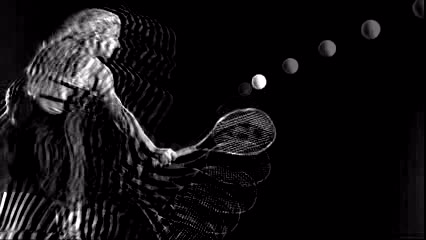
\includegraphics[width=0.9\columnwidth]{imagenes/cualitativos/TAS.png}
\end{center}
\end{figure}
\FloatBarrier

\par Si bien la presencia de este tipo de artifacts no implica necesariamente un error en los algoritmos, nos llam\'o la atenci\'on.
Revisamos nuestros tests y notamos que no contemplamos en ninguno ciertos casos donde la cantidad de frames no es divisible por el tama\~no de bloques.
Agregamos tests que cubran estos casos y efectivamente, nuestra implementaci\'on de Splines no los pasaba.
Repasamos nuestro c\'odigo, cotejando con bibliograf\'ia de la materia\cite{Burden}, y notamos una discrepancia;
al arreglar el error, los tests pasaban y desapareci\'o el artifact detallado previamente.
Debido a esto, consideramos la implementaci\'on correcta.
